\chapter{Resultados}\label{chp-07}

\lettrine[lraise=-0.1, lines=2, loversize=0.2]{F}inalmente, aunando todo el desarrollo expuesto en los capítulos precedentes se expone en este capítulo el resultado del trabajo y su conversión del campo teórico a la práctica, llegando a construir de forma real el dispositivo de control.

\section{Placas}

Siguiendo con el diseño electrónico se han fabricado las placas electrónicas necesarias para el proyecto.
En la figura \ref{fig:placafondo} y en la figura \ref{fig:placatapa} se muestran las placas con sus pistas y sus componentes soldados.

\begin{figure}[hbtp]%  
    \centering 
        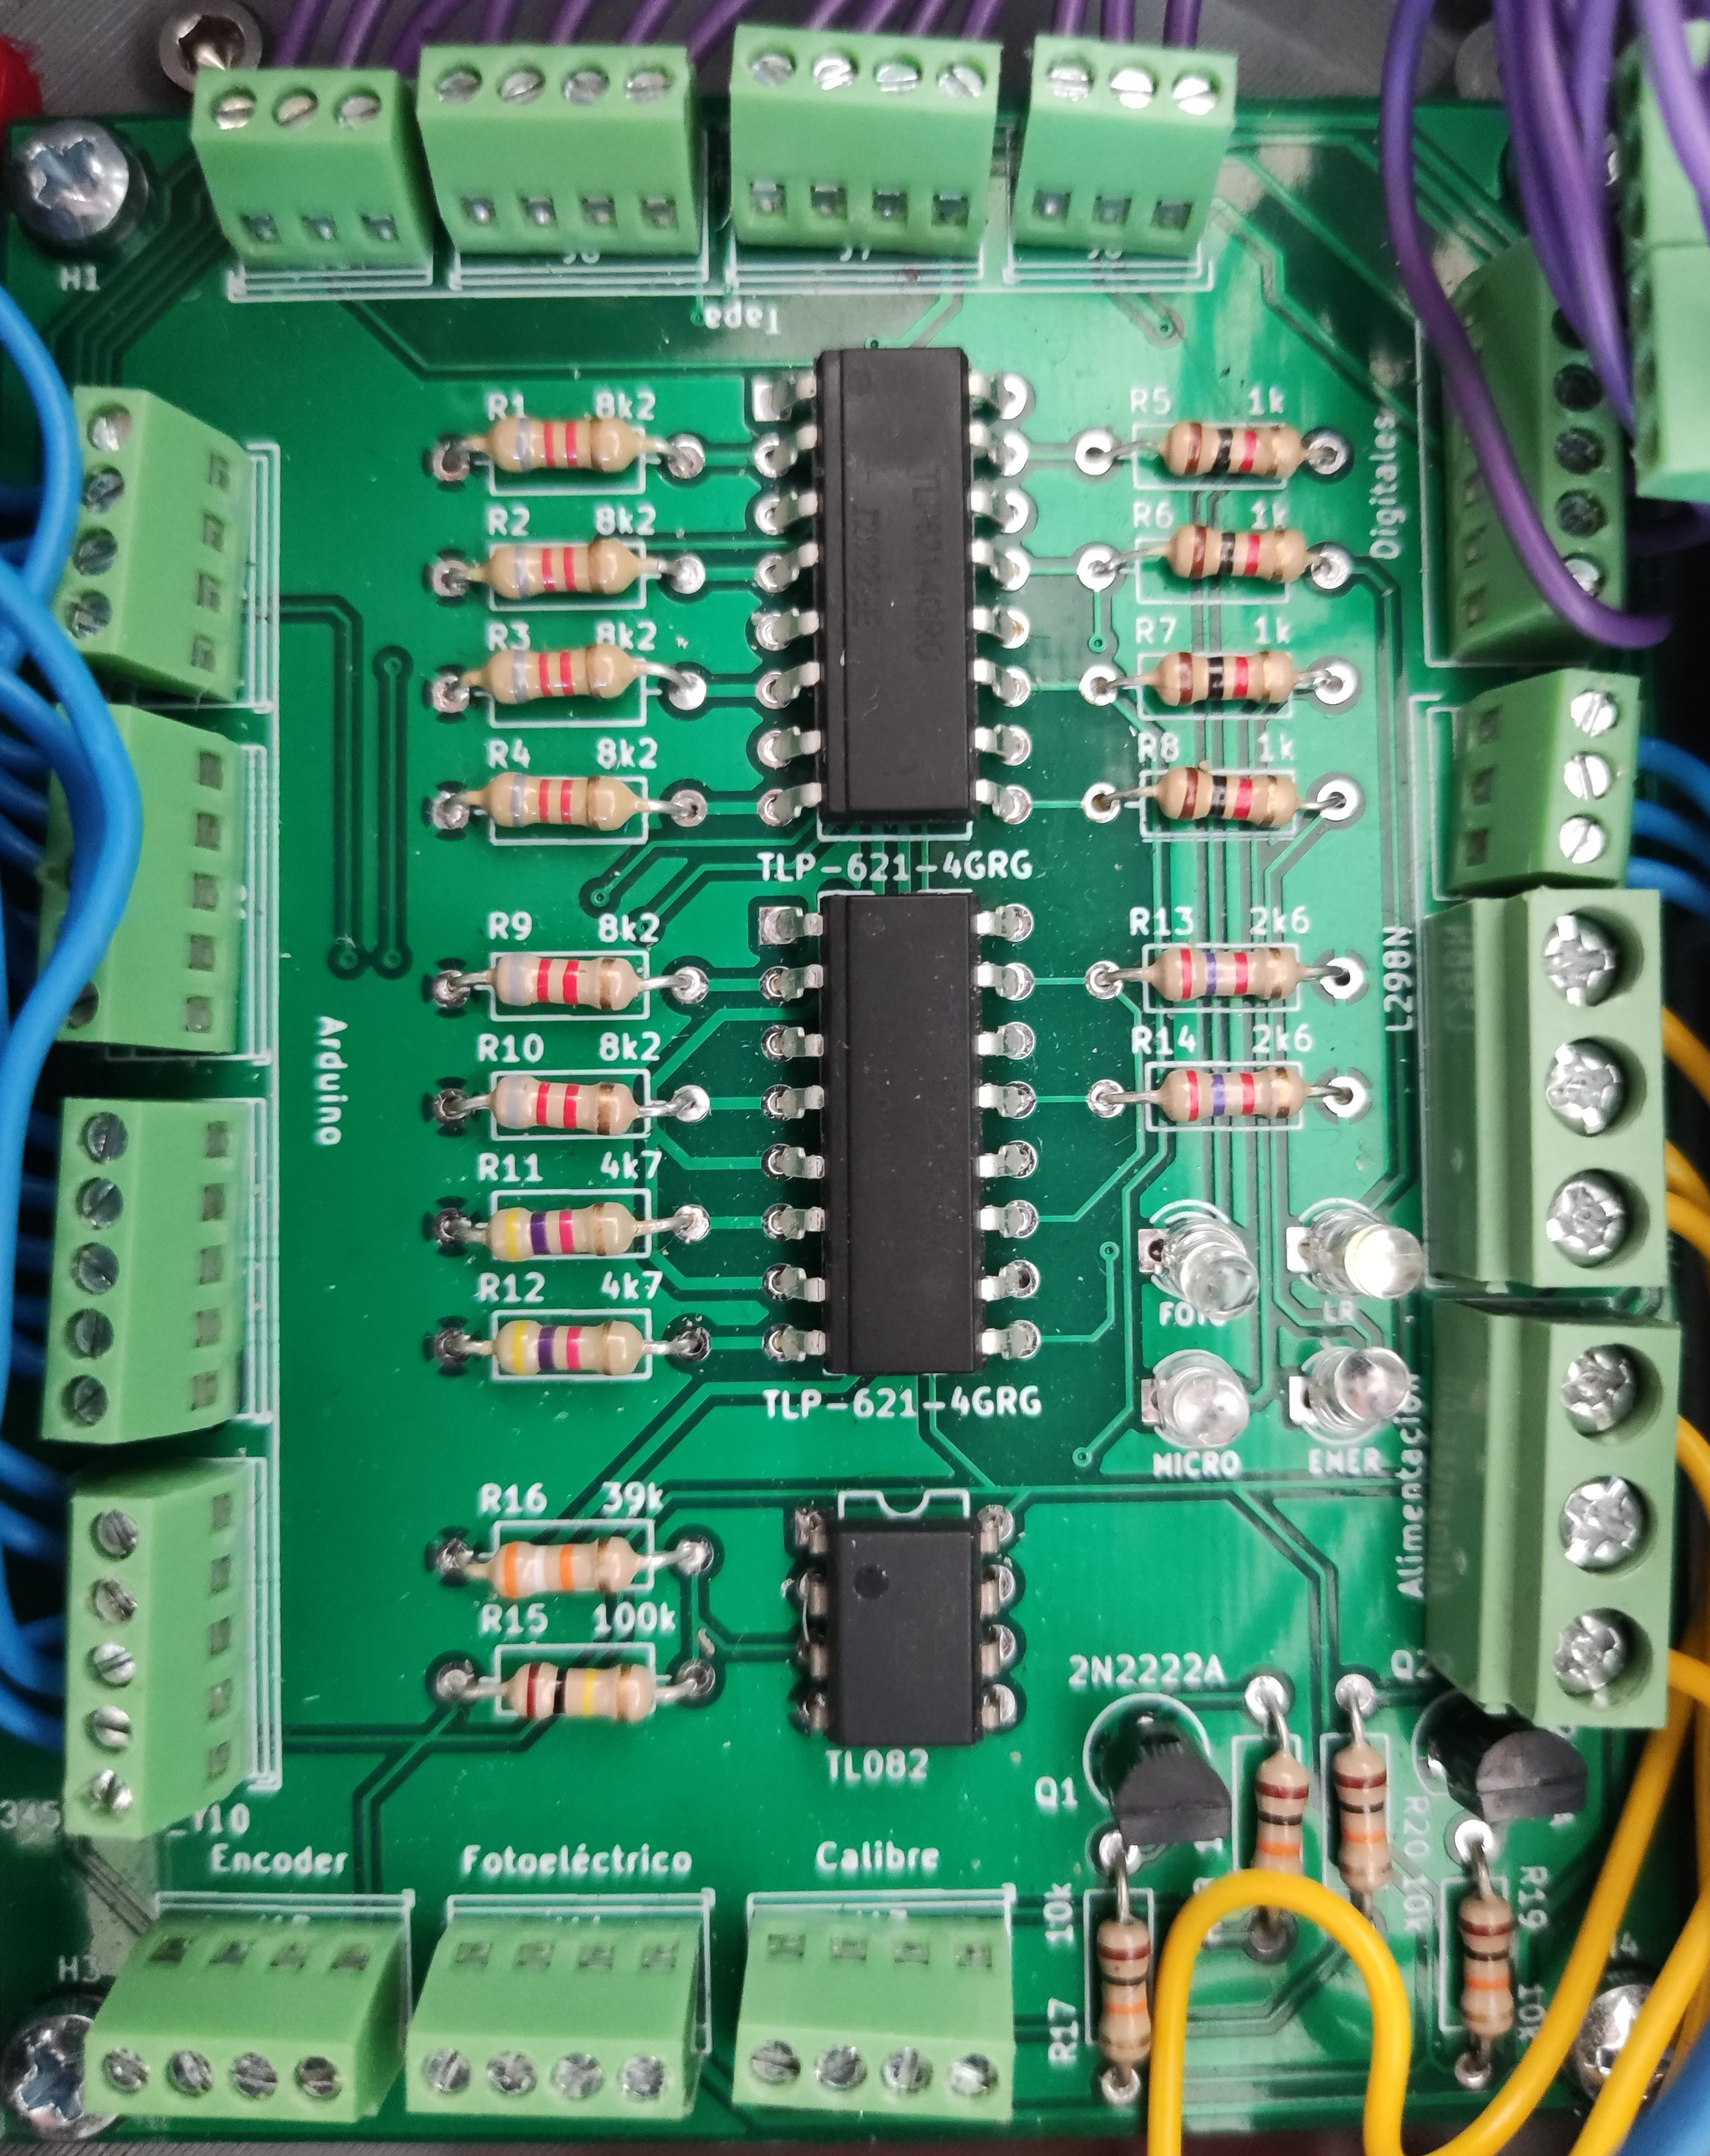
\includegraphics[width=0.33\textwidth]{07-resultados/placafondo.jpg}
    \caption{Placa de conexiones general}
    \label{fig:placafondo} 
\end{figure}

\begin{figure}[hbtp]%  
    \centering 
        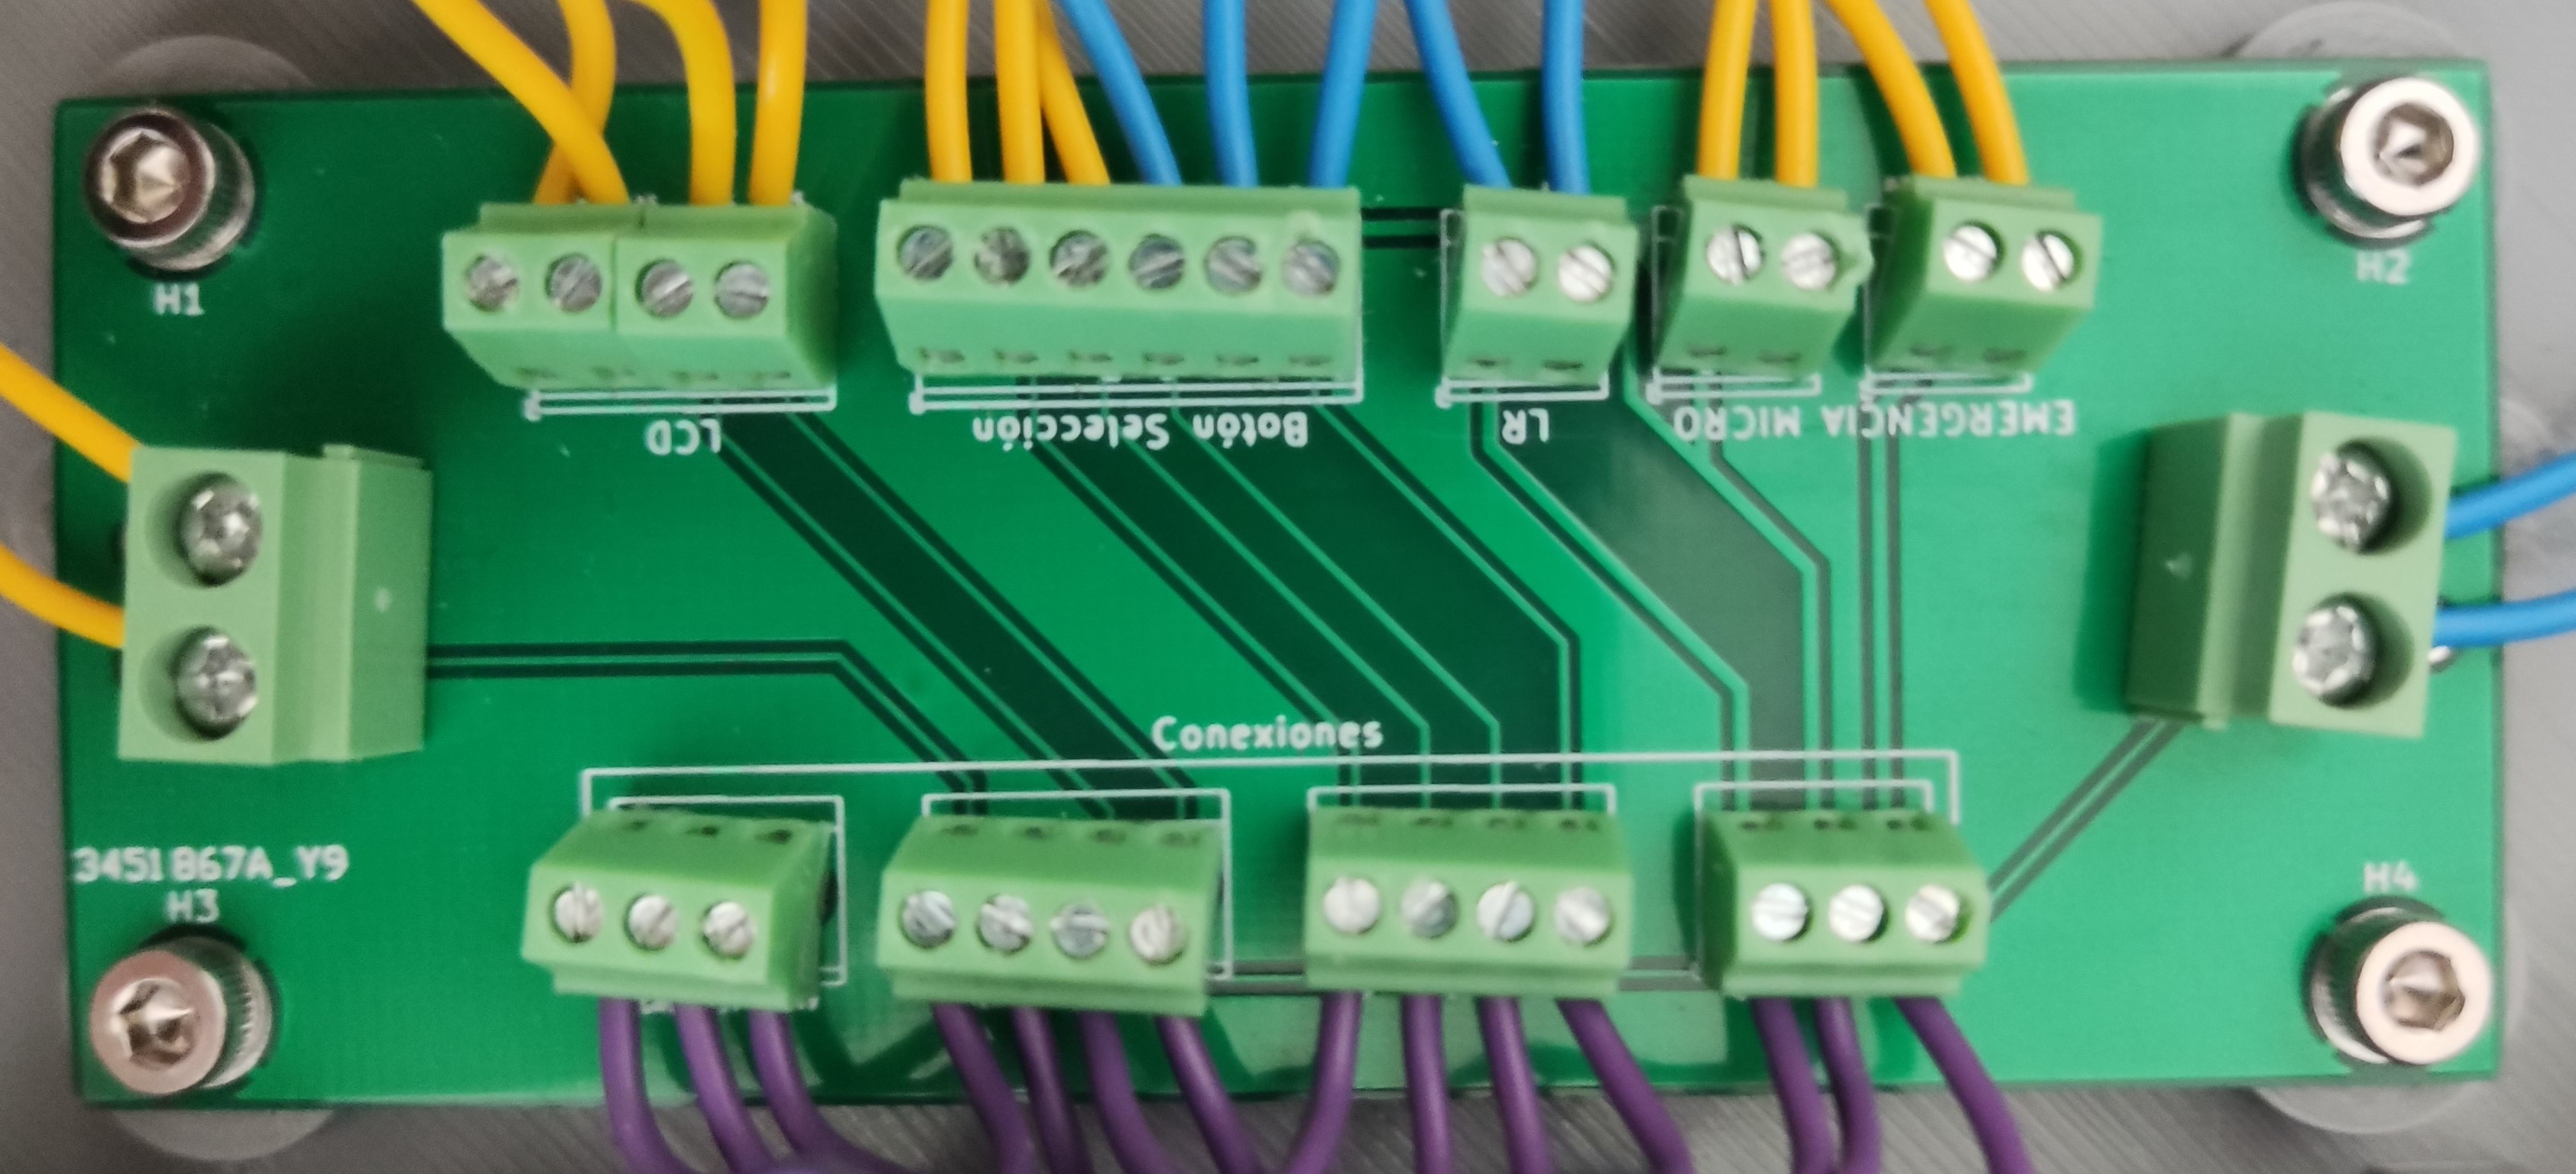
\includegraphics[width=0.4\textwidth]{07-resultados/placatapa.jpg}
    \caption{Placa de conexiones de la tapa}
    \label{fig:placatapa} 
\end{figure}

\section{Panel de control}

La caja que contiene los elementos del panel de control se ha impreso en 3D y se ha ensamblado. En la figura \ref{fig:cajaexterior} se muestra en perspectiva el panel de control con todos sus elementos unidos, tanto la base como la tapa. Además se muestra la interfaz de usuario al completo.

\begin{figure}[hbtp]%  
    \centering 
        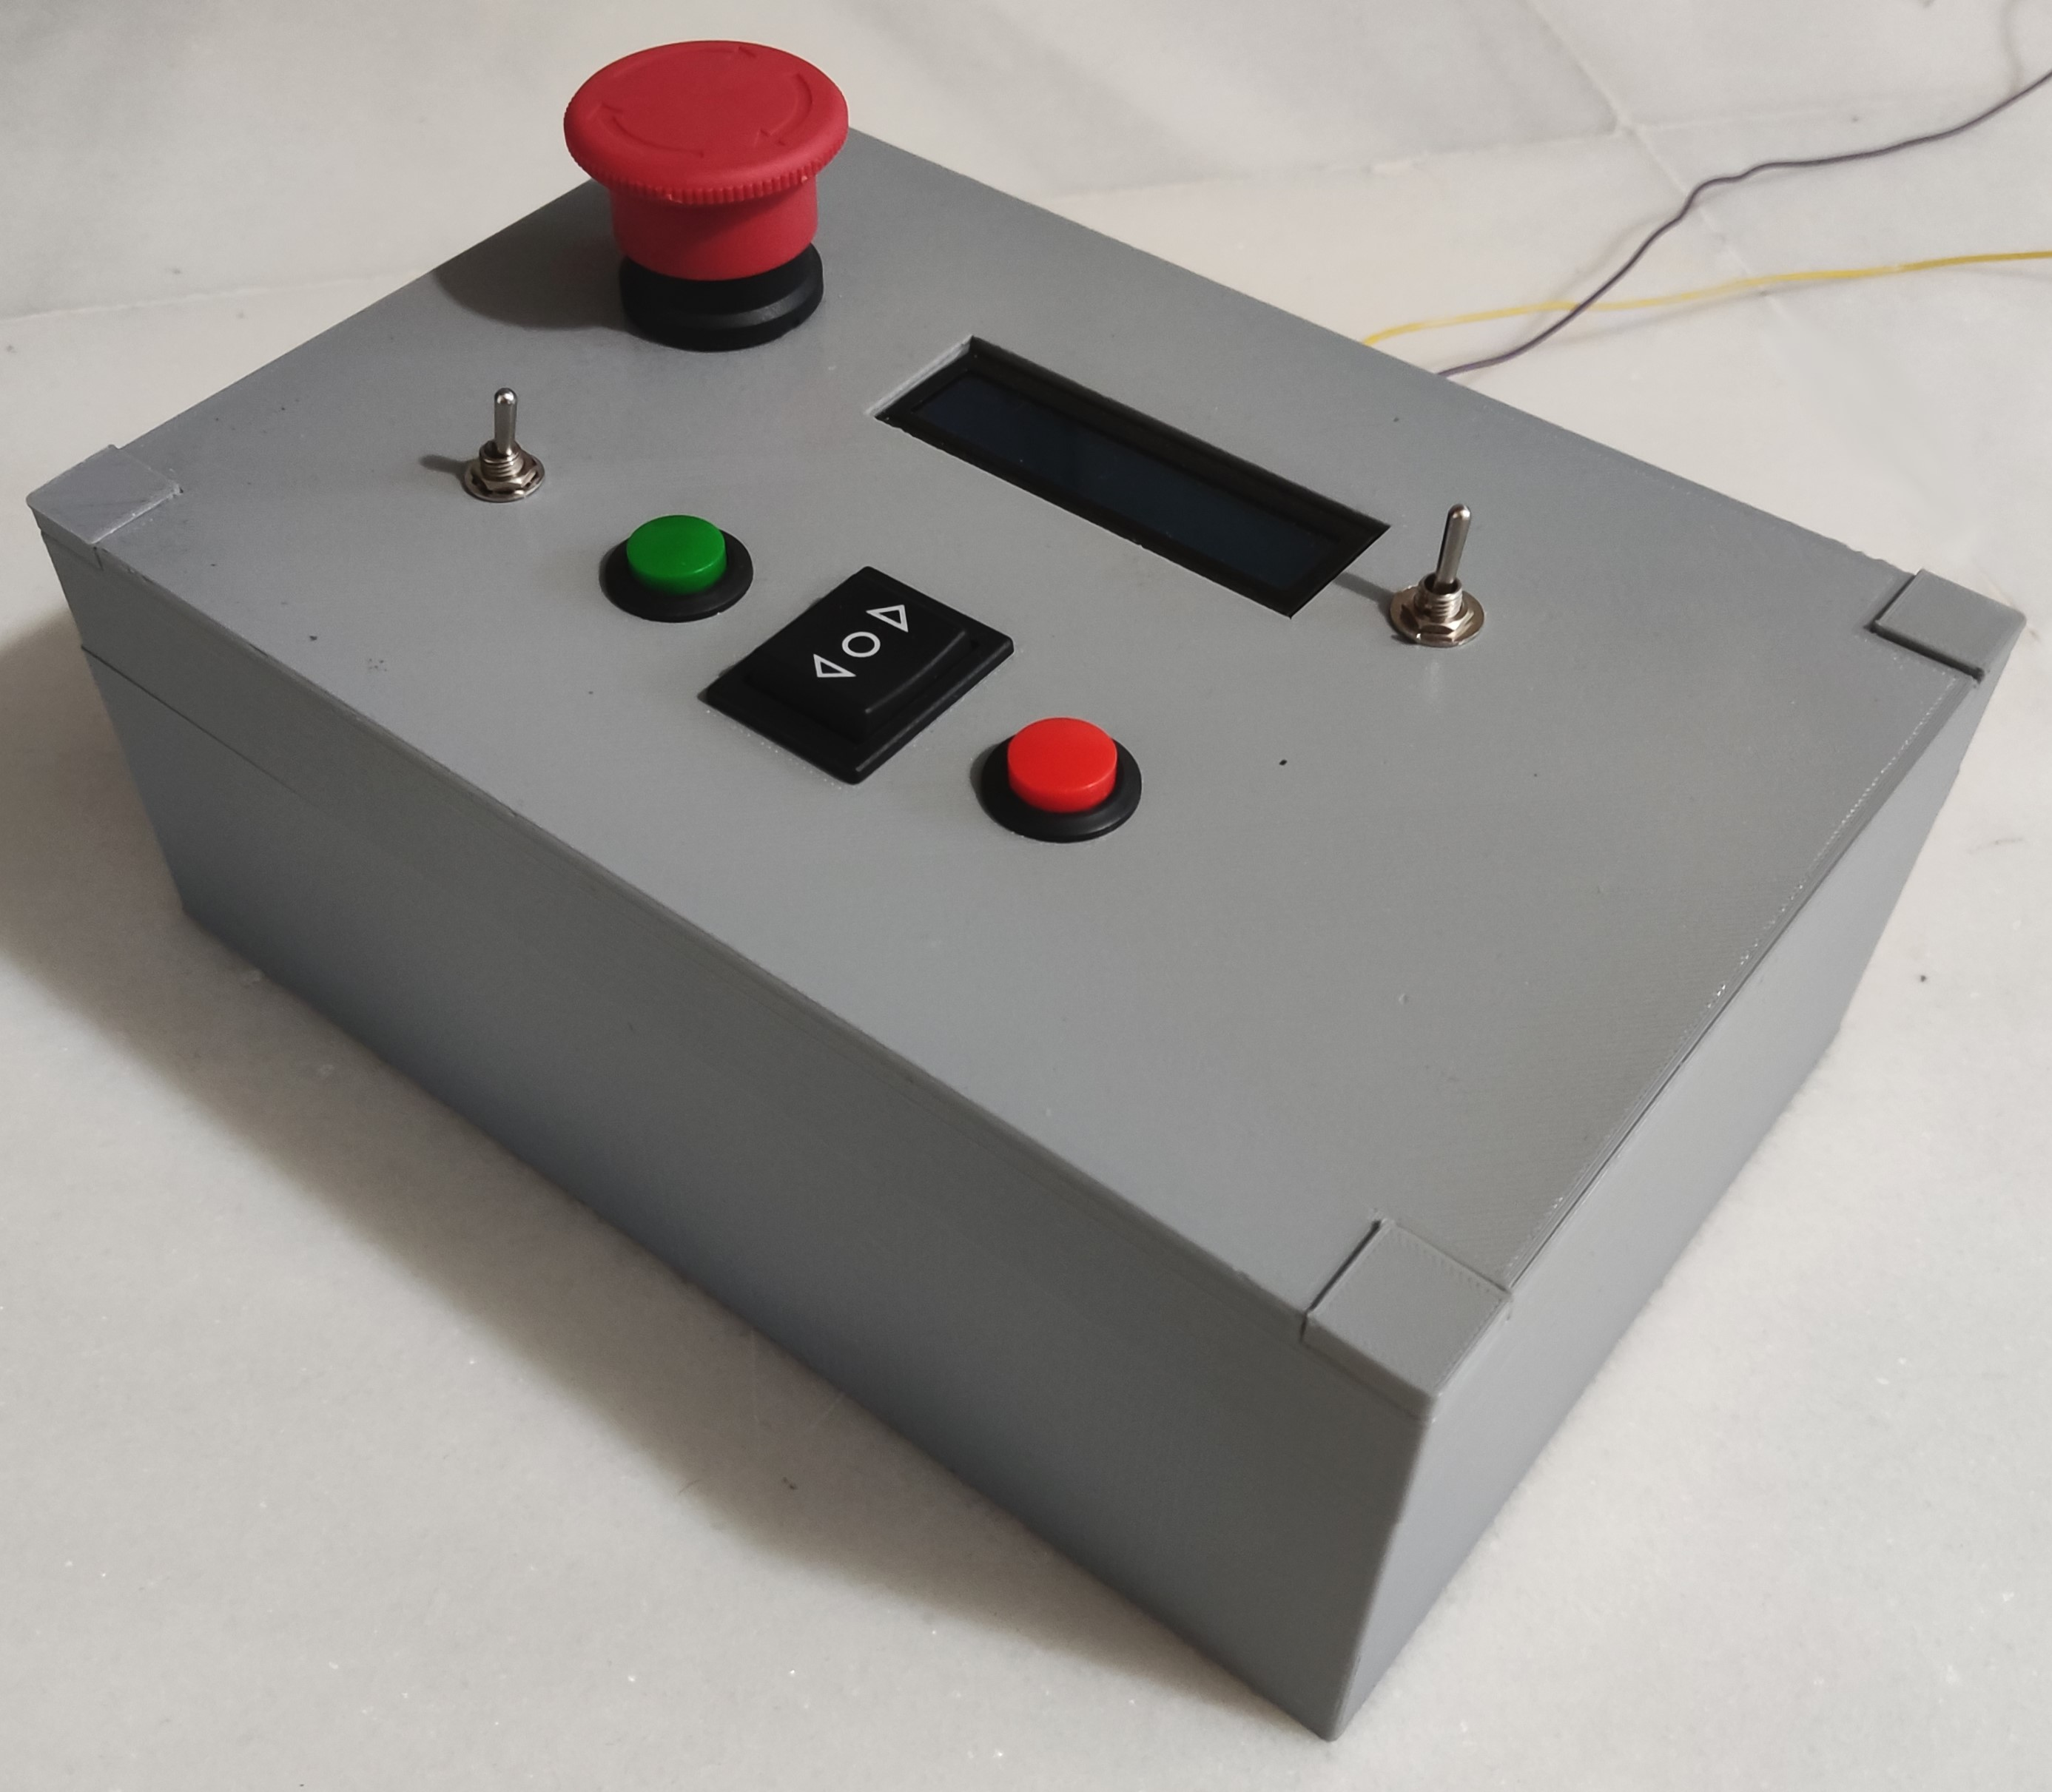
\includegraphics[width=0.55\textwidth]{07-resultados/cajaexterior.jpg}
    \caption{Vista en perspectiva del panel de control}
    \label{fig:cajaexterior} 
\end{figure}

En la figura \ref{fig:cajatrasero} se muestra la parte trasera de la caja, donde se encuentra
el orificio donde se introducen los cables, el conector Ethernet y los pines digitales.

\begin{figure}[hbtp]%  
    \centering 
        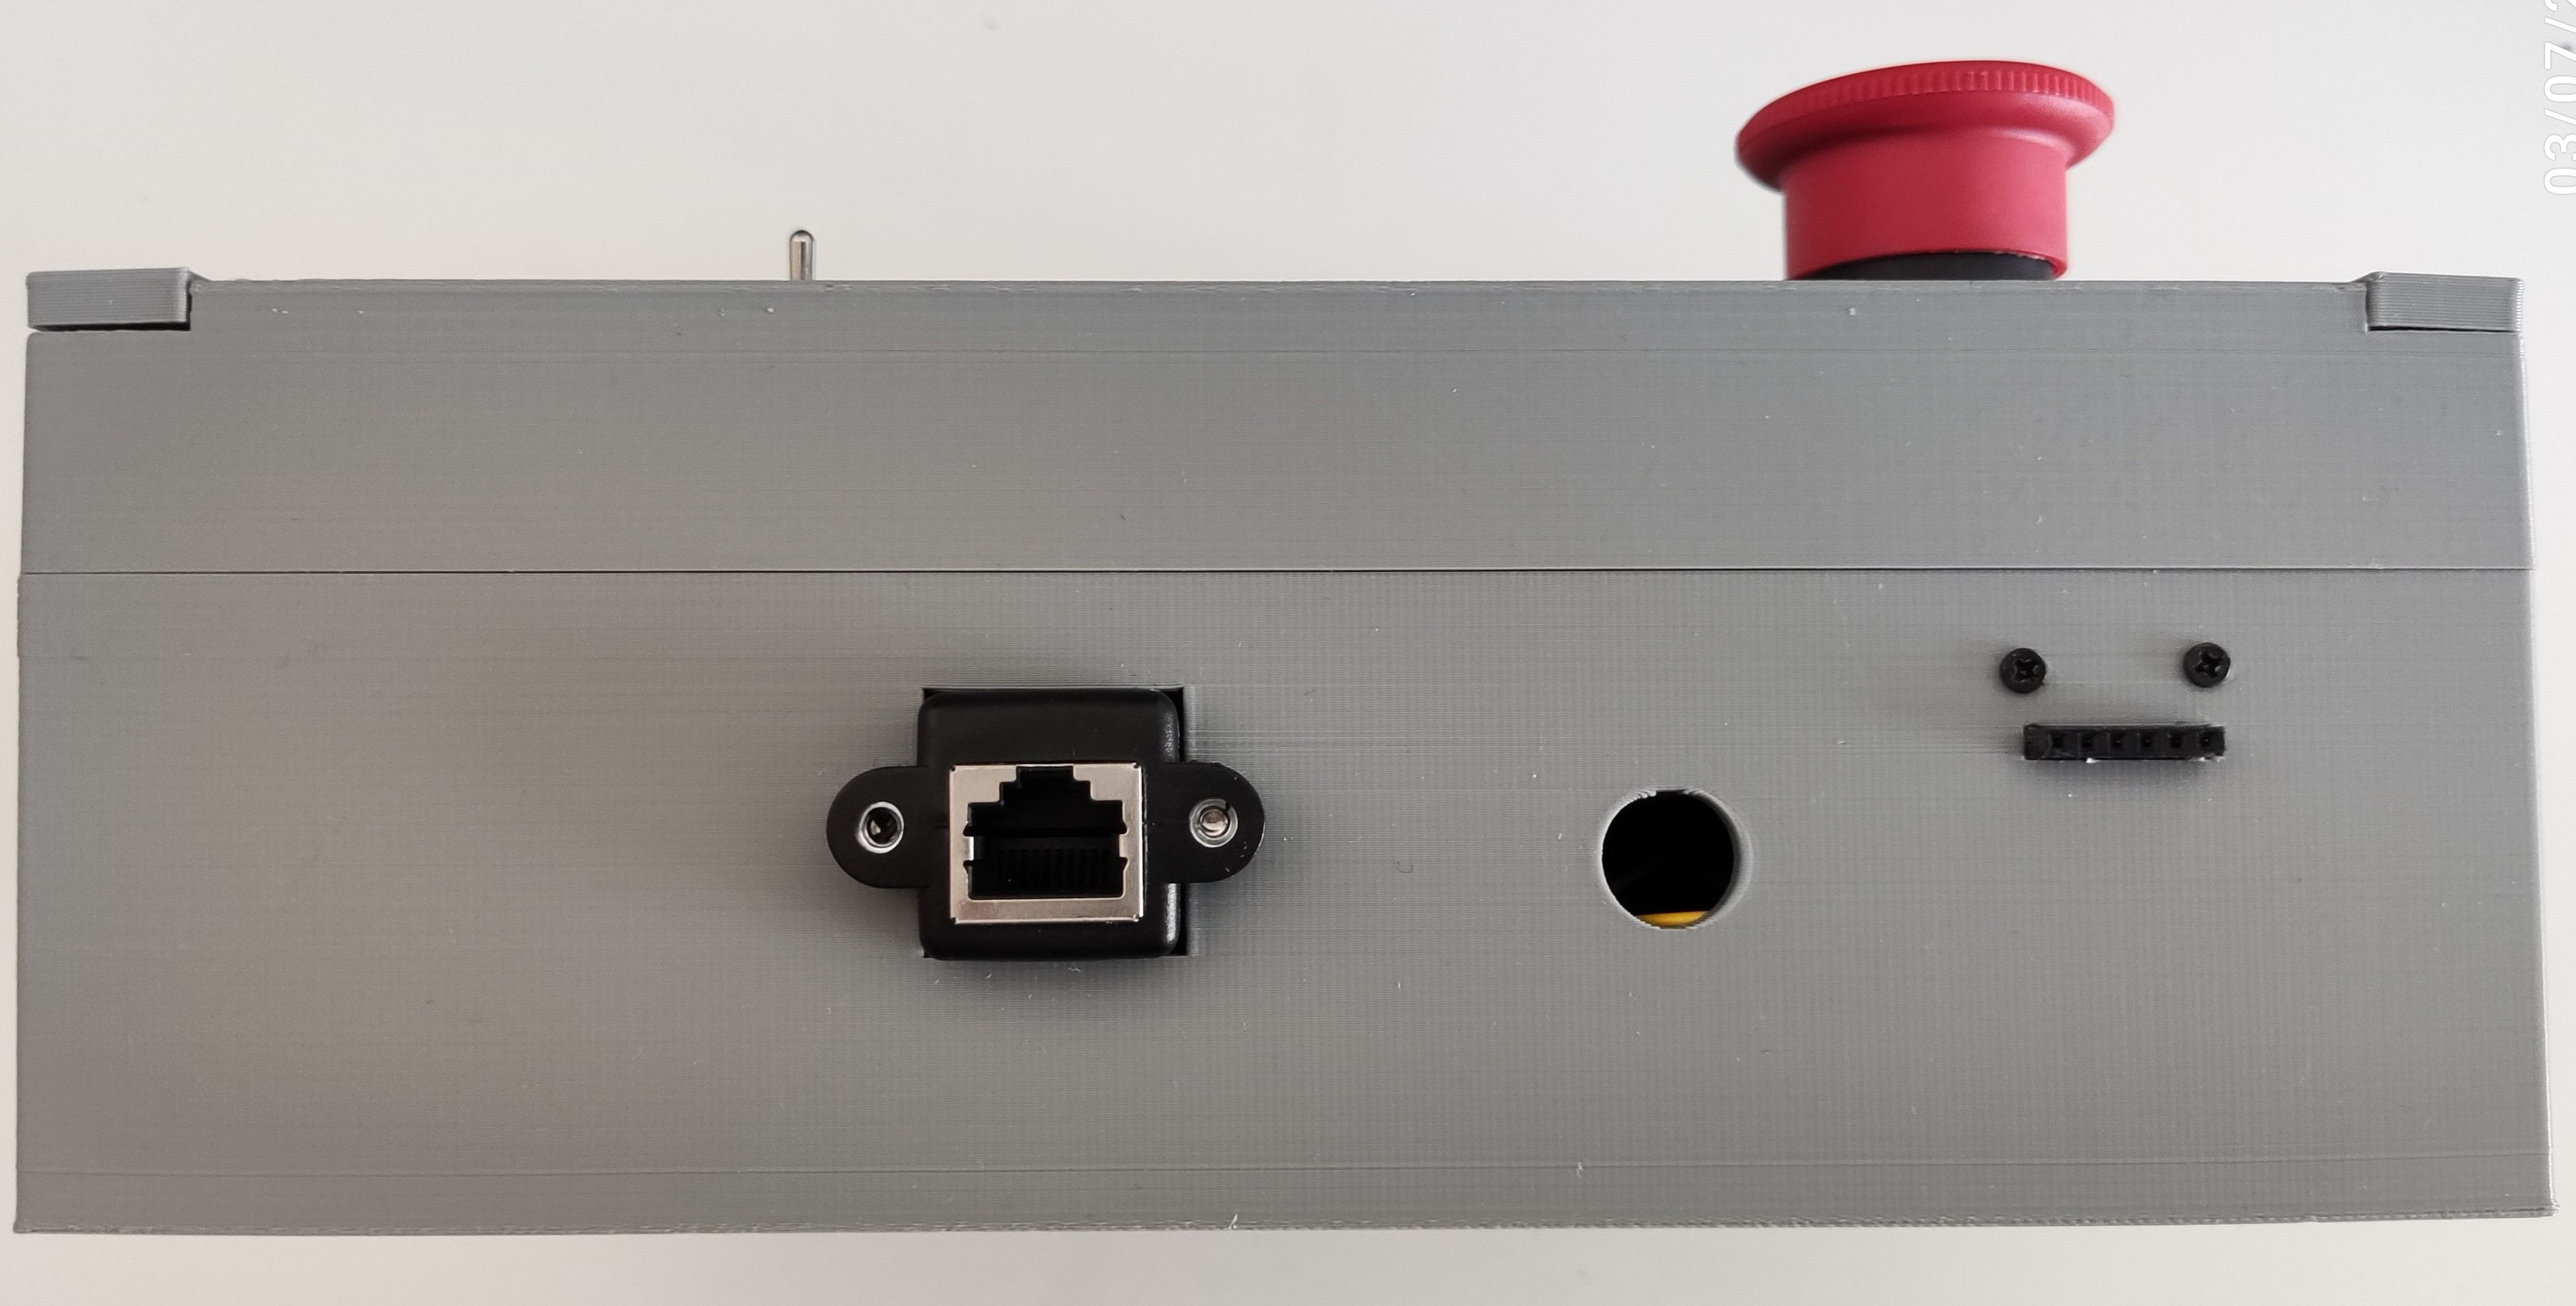
\includegraphics[width=0.75\textwidth]{07-resultados/cajatrasero.jpg}
    \caption{Vista trasera del panel de control}
    \label{fig:cajatrasero} 
\end{figure}



\section{Integración de componentes}

Una vez fabricadas la caja del panel y las placas electrónicas, se integran todos 
los dispositivos y se realizan las conexiones pertinentes. En la figura \ref{fig:cajainterior}
se muestra el interior de la base del panel, con todos los cables y conexiones internas.

\begin{figure}[hbtp]%  
    \centering 
        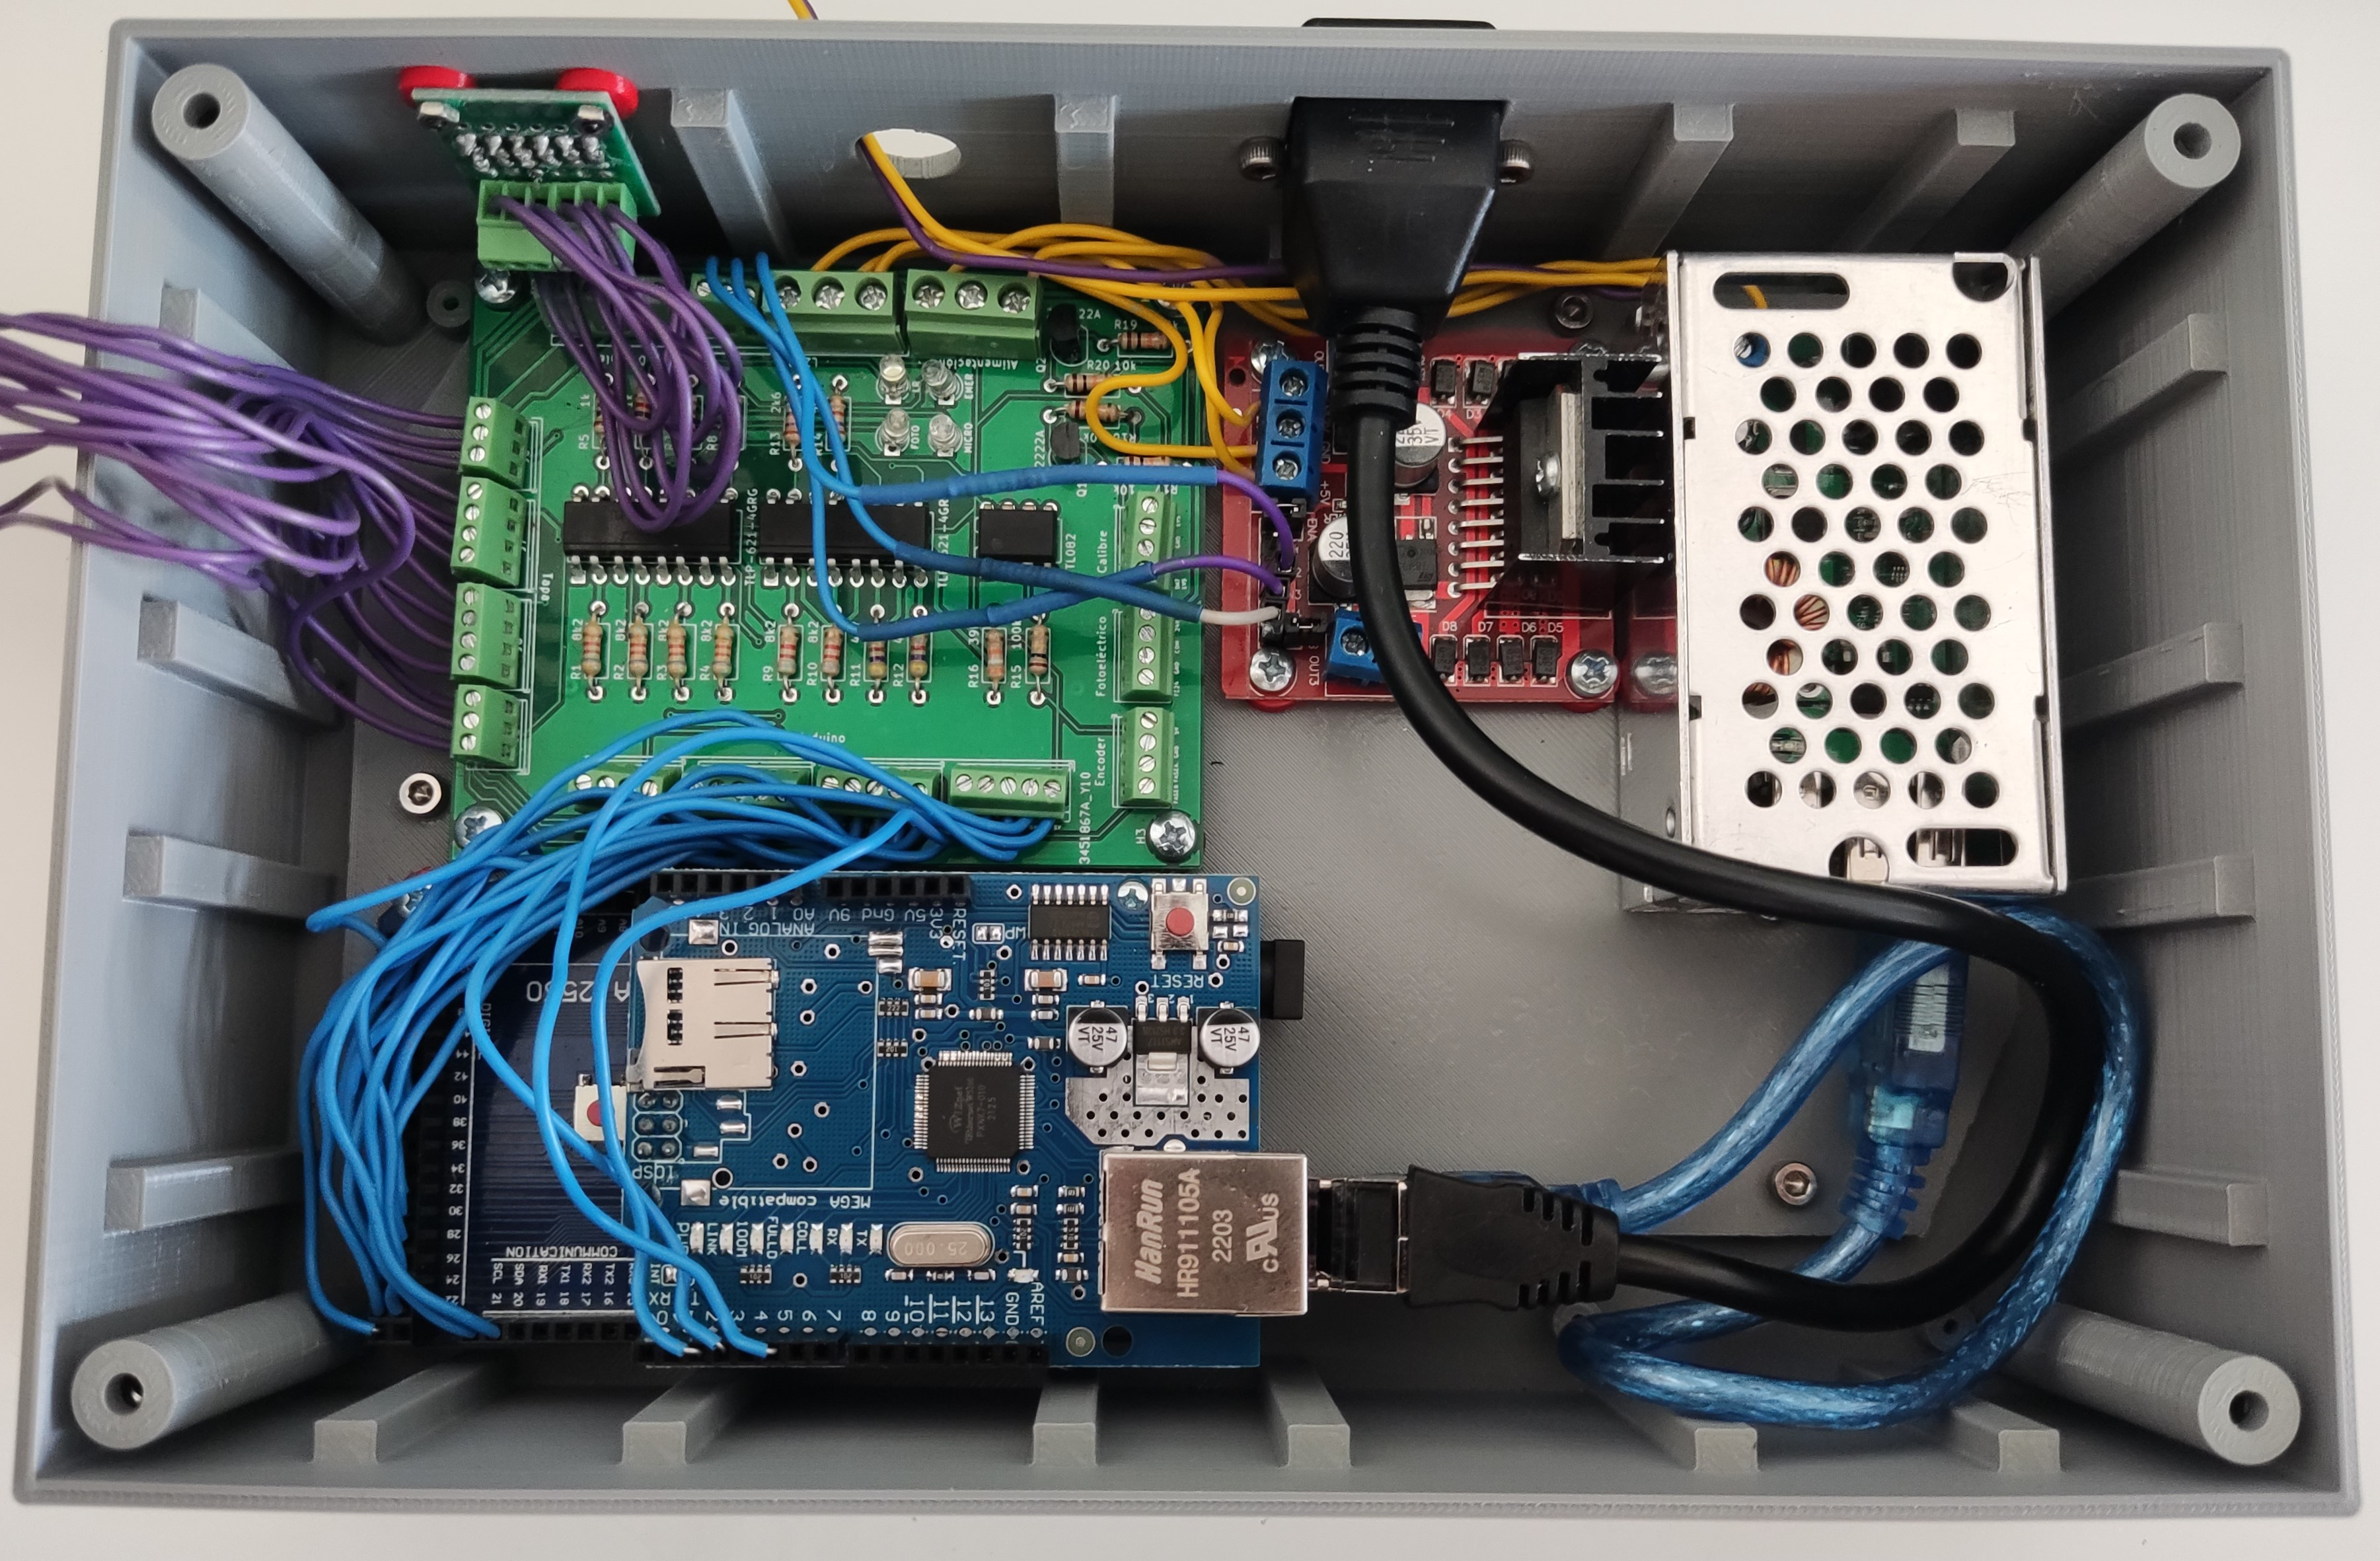
\includegraphics[width=0.75\textwidth]{07-resultados/cajainterior.jpg}
    \caption{Interior de la base del panel con todos sus componentes}
    \label{fig:cajainterior} 
\end{figure}

Por otro lado, en la figura \ref{fig:cajatapainterior} se muestra el interior de la tapa del panel, mostrando cómo están conectados los botones, los interruptores, la seta y el LCD.

\begin{figure}[hbtp]
    \centering 
        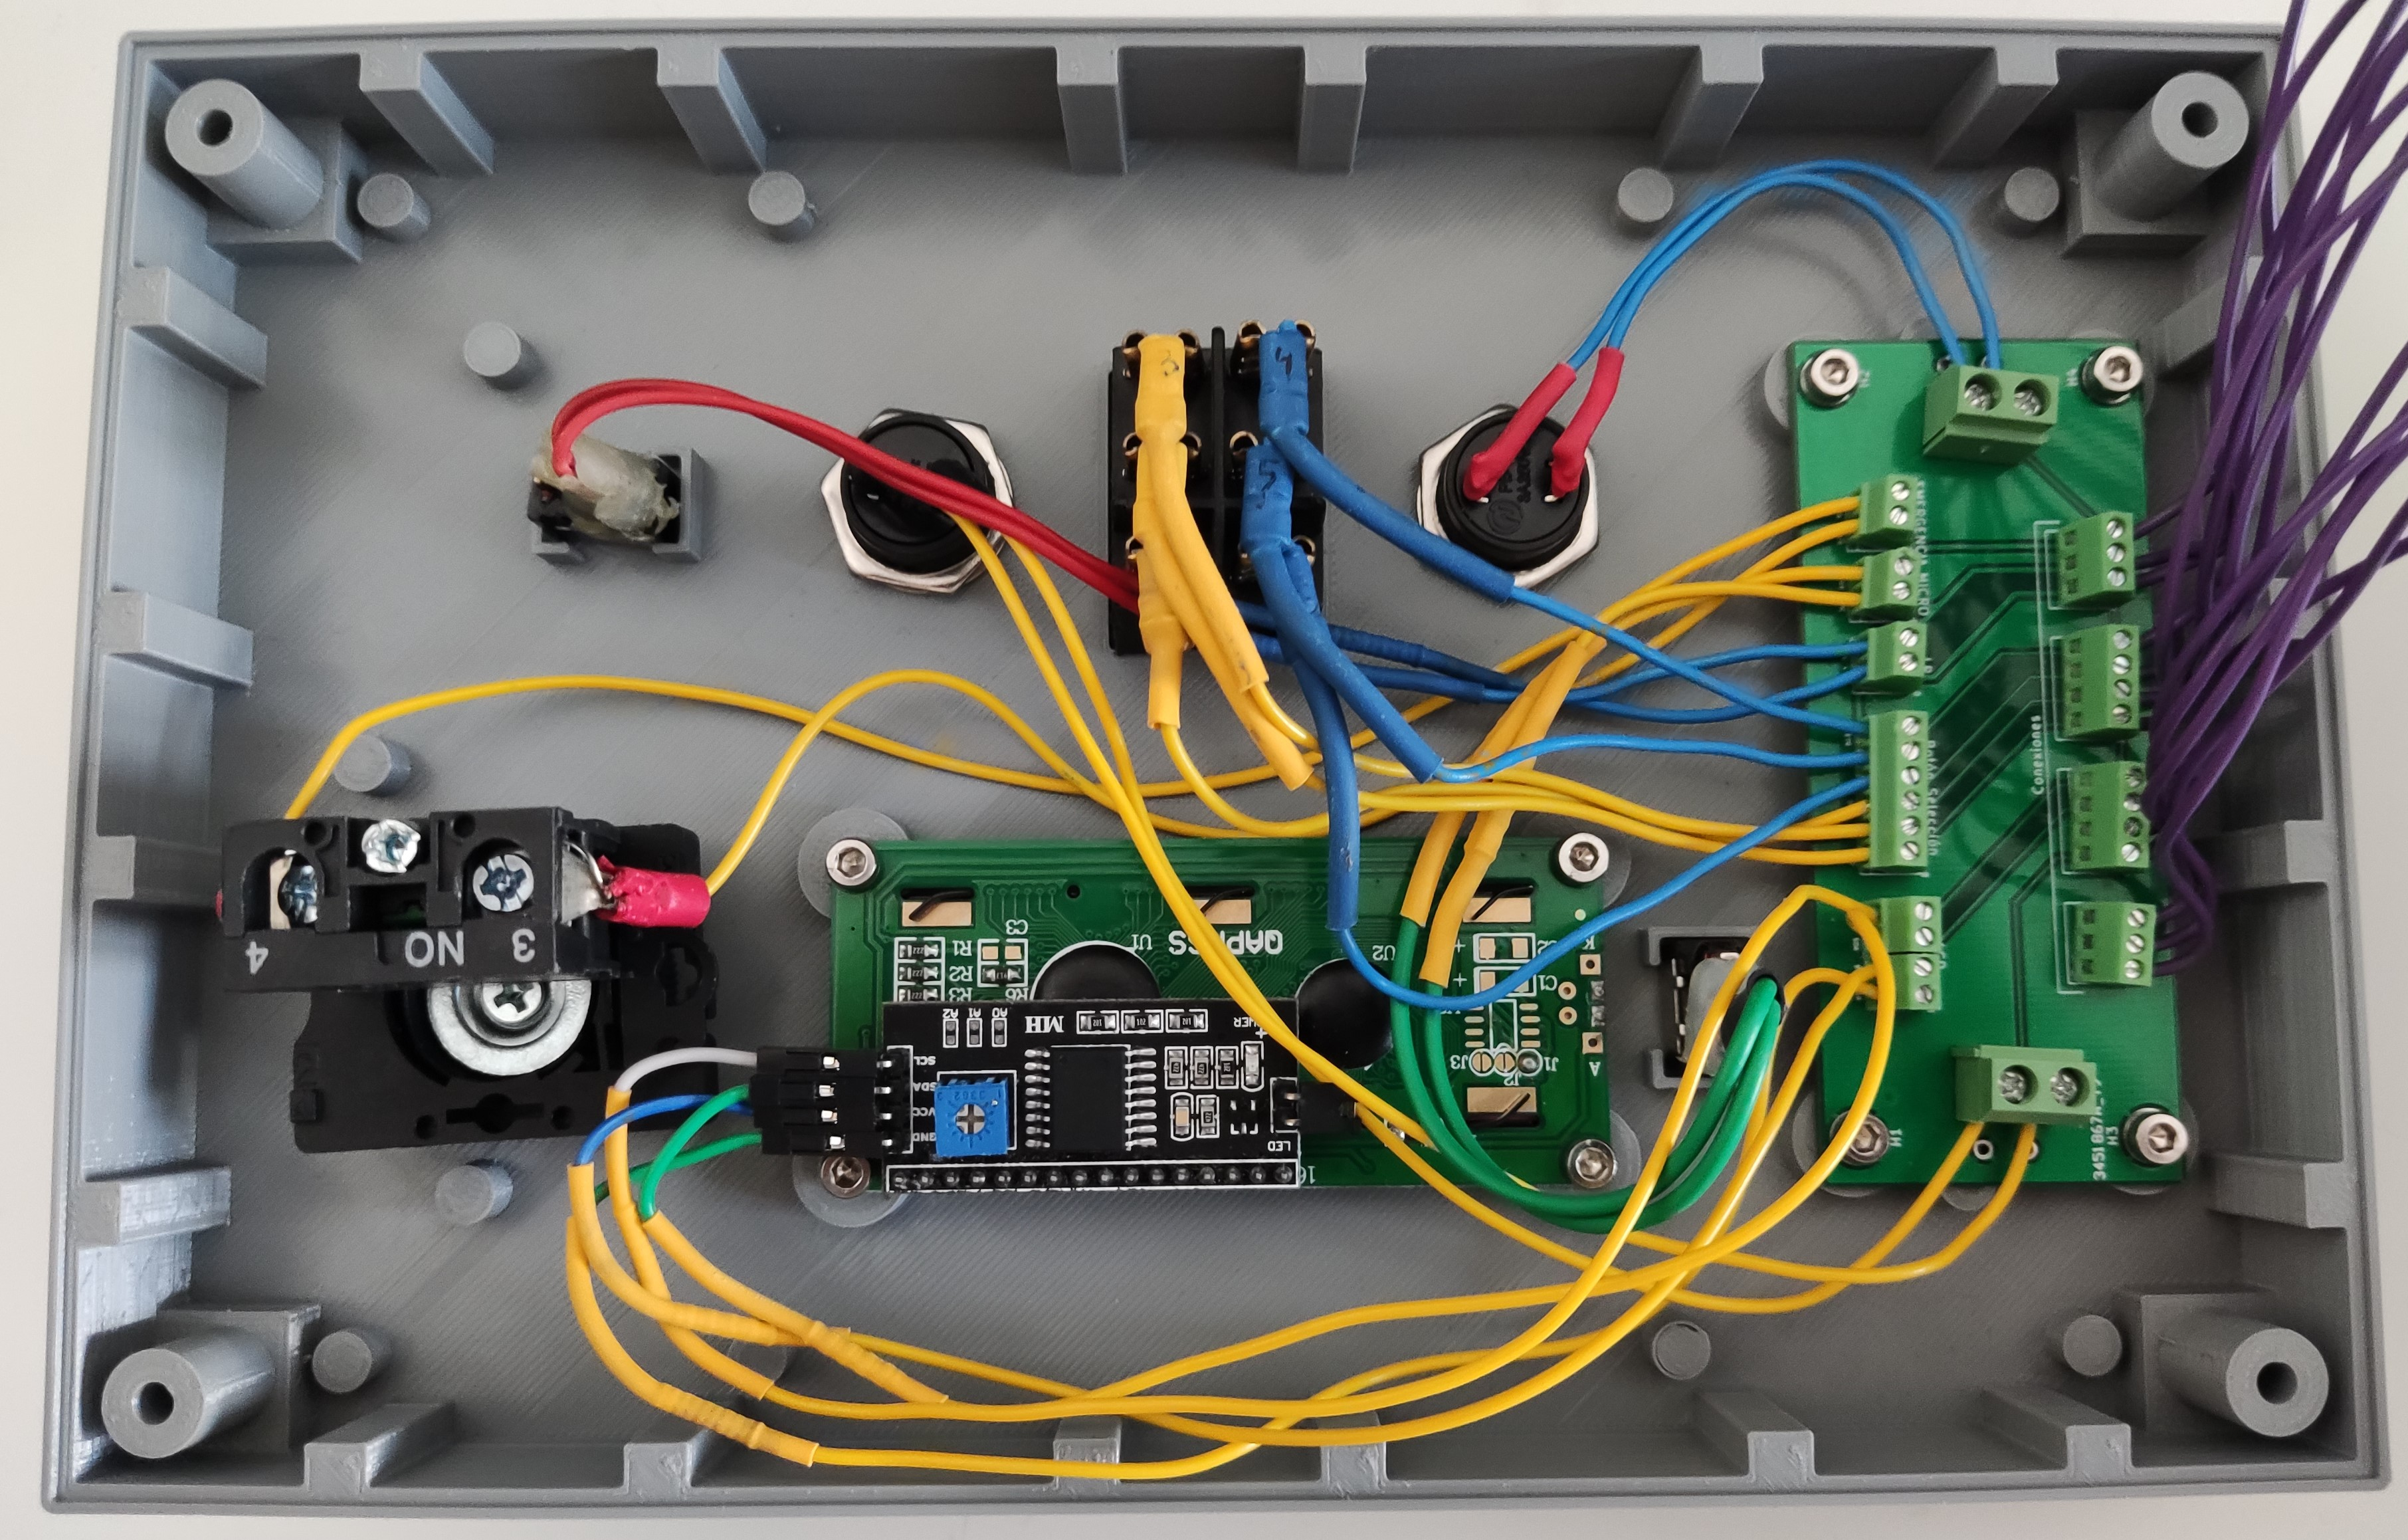
\includegraphics[width=0.75\textwidth]{07-resultados/cajatapa.jpg}
    \caption{Interior de la tapa del panel con sus componentes}
    \label{fig:cajatapainterior} 
\end{figure}
